This chapter gives an overview of our approach for building the JS-QL framework. For this framework we used the JIPDA static analysis tool to generate an abstract state graph representing a JavaScript program. This graph contains control- and value-flow information, necessary to detect more complex security vulnerabilities. We have developed JS-QL, a querying language to effectively query for security vulnerabilties in JavaScript programs. The language is built as an internal domain-specific language on top of JavaScript. Our approach combines the JIPDA abstract state graph with JS-QL, resulting in a tool in which application-specific and user-defined security policies can be specified and checked.

\section{Architecture}
\label{sec:Architecture}

The actual architecture of the JS-QL framework is depicted in figure \ref{fig:architecture}. The query engine takes as input (i) a flow graph and (ii) a query, written in the JS-QL language. The output will consist of tuples \texttt{<State, Substitutions>} for all paths on which a match for the query was found.

\begin{figure}
    \centering
      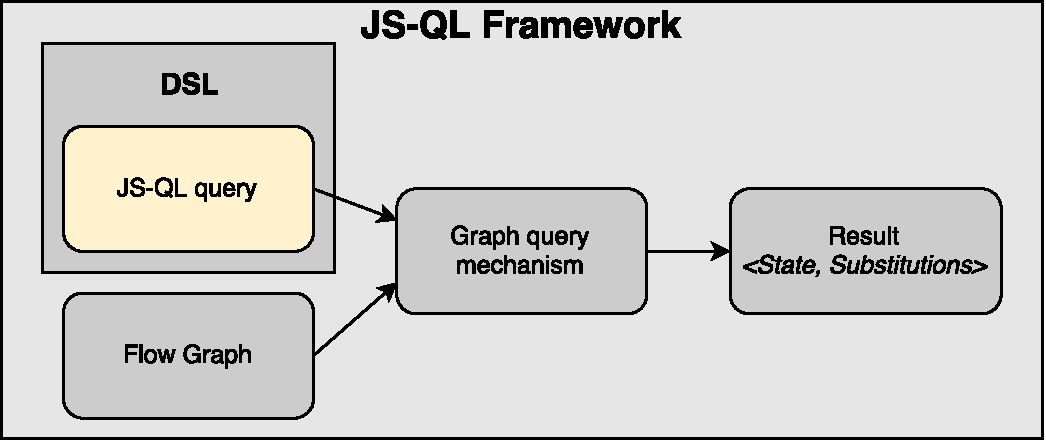
\includegraphics[width=0.9\textwidth]{images/Architecture} 
      \caption{JS-QL framework architecture}
    \label{fig:architecture}
\end{figure}

%program representation
\subsection*{Program representation}

For our approach, we used static analysis to represent a JavaScript program as a graph. Abstract interpretation, a static analysis technique, produces an abstract state graph when given a program as input. The graph contains information about control- and data flow, providing a rich source of information that can be extracted through some query language and a querying mechanism. 

There is an extensive body of related work on how logical programming can be used to represent and analyse programs\cite{Reps1995}\cite{DatalogDBQueries}. However, static analysis combined with a query language leans more closely towards the implementation of our system.  As discussed in section \ref{sec:staticAnalysis}, static analysis can be a means of representing implicit and explicit information about source code. 

\subsection*{Query mechanism}

Program querying depends on the way a program is represented and how queries are transformed into query-engine-friendly data structures. Our approach represents programs as flow graphs, and queries against these graphs need to be resolved. A suitable algorithm for solving queries is presented in \cite{algoEngine}, which enables us to query flow graphs directly. The internals of this algorithm will be discussed in greater detail in section \ref{sec:matchingEngine}. An alternative approach would be to use existing techniques such as \textit{bddbddb}\cite{bddbddb}. This technique matches queries expressed in Datalog against a database of rules representing the relations of an entire program. The overhead for this approach would however be too large, as we would have to transform the abstract state graph to Datalog rules.

\subsection*{Query language}
% DSL
With the JS-QL language, we offer an internal domain-specific language specialized in expressing queries corresponding to sequences of states in the flow graph. The language makes use of \textit{regular path expressions}, which are expressions describing the path that needs to be traversed in a graph in a syntax similar to regular expressions.It is important that exploring and accessing information of a flow graph happens in a user-friendly way, as such graphs might be complex to understand. We believe that regular path expressions enable users to write clean and understandable queries. 


\section{Flow graphs for JavaScript programs}
\label{sec:FlowGraphs}
The need for detailed control- and data flow information in our program representation graph limits the types of graphs that can be used for our framework. The JIPDA\cite{functionPurity} abstract state graph, generated by statically analyzing source code through \textit{abstract interpretation}, contains all the information needed to precisely express patterns to be detected in a program. The JS-QL framework uses the JIPDA graph as its program representation. This section takes an in-depth look at the JIPDA abstract state graph and the information it holds in its states. Other flow graphs, such as program dependence graphs\cite{PDG}, can be useful to track the flow of information between certain points in a program, but often lack more general information about program states, making them less qualified to use as our main program representation.

\subsection{Information in an abstract state graph}

Figure \ref{fig:JipdaGraph} shows part of a typical graph produced by JIPDA for a program containing a check for whether a number is equal to zero or not. As can be observed, the graph depicts all possible paths a program can traverse. Since the analysis in JIPDA is flow-sensitive, it is guaranteed that a state \texttt{a} on some path in the graph occurs before a state \texttt{b} on the same path if state \texttt{a} occurs before state \texttt{b} on the path. This makes reasoning about patterns in a program much easier, since no false positives will occur with regards to the order of execution of states. The graph produced by the JIPDA analysis is also a flow graph, and more precisely maintains information about two types of flows:

\begin{figure}[!ht]
    \centering
      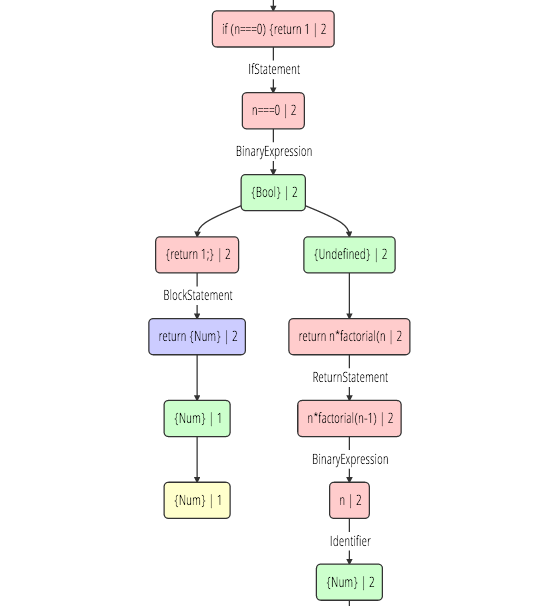
\includegraphics[width=262px, height=606px, keepaspectratio]{images/JipdaGraph} 
      \caption{Example JIPDA abstract state graph}
    \label{fig:JipdaGraph}
\end{figure}

\begin{enumerate}
\item \textit{Data flow}: Information about what values an expression may evaluate to.
\item \textit{Control flow}: Information about which functions can be applied at a call site.
\end{enumerate}

\noindent We need this information to be able to make correct assumptions at certain states in a program, as illustrated in example \ref{ex:cdflow}. 

\begin{exmp}
\label{ex:cdflow}
Consider the expression \texttt{f(x)}. Function \texttt{f} will be the function that is invoked. The value of \texttt{f} however may depend on other operations that occur before this function call, such as another function call. Therefore it is important to know which function(s) \texttt{f} may refer to, illustrating the need of control and data flow.
\end{exmp}

\subsection{States of an abstract state graph}

JIPDA uses Esprima\cite{Esprima} to parse JavaScript code and set up an abstract syntax tree (AST). This AST is the starting point for the analysis that JIPDA performs, hence information about the nodes from the AST is also contained in certain states in the resulting graph. The small-step semantics of a program are defined by an abstract machine that transitions between different states. The abstract machine is in eval-continuation style, indicating that a state is either an evaluation state or a continuation state. These states correspond to the states that can be seen in the abstract state graph. The states the machine can be in are described below:

\begin{enumerate}
\item \textit{Evaluation state}: Represents the evaluation of an expression of the program in the binding environment $\beta$.
\item \textit{Continuation state}: A state which indicates that the machine is ready to continue evaluation with the value it just calculated.
\item \textit{Return state}: This is a special kind of continuation state, as it indicates the return of a function application. When the machine is in this state it is ready to continue evaluation with the value calculated for the return of the function application.
\item \textit{Result state}: The final state of the graph, indicating the final computed value(s) of the program. This is also a special kind of continuation state. The machine and graph can have more than one result state, depending on the program's nature. 
\end{enumerate}



%Kont, Lkont, Node, Benv, Store, Value
\subsection{Attributes of the states}
These states all contain relevant information about the point in the program they represent. The next part of this section discusses the different attributes that can be found in the states of the abstract state graph. 

\subsubsection*{Node}

Evaluation states contain information about the expression or statement they represent in the program. This information is stored in the form of an AST node, as obtained by the Esprima parser. Detailed information about the current expression or statement can be found in the properties of these nodes. Our approach makes extensive use of this information to find a match for a specified pattern along the graph. Note that node information is exclusively available in evaluation states. Example \ref{ex:answerUniverse} depicts the layout of the AST-tree for a trivial JavaScript program.

\begin{exmp}
\label{ex:answerUniverse}
If we parse the following program \\\\
\texttt{function answerToTheUniverse(arg)\{}\\
\phantom{ }\phantom{ }\phantom{ }\phantom{ }\texttt{return 42;}\\
\texttt{\}}\\
\\
we obtain its corresponding JSON representation, listed in \ref{lst:EsprimaTree}.
\\
\begin{lstlisting}[label={lst:EsprimaTree},language=JSON,caption=Parsed JavaScript program AST, mathescape=true]  % float=t?

{
    "type": "Program",
    "body": [
        {
            "type": "FunctionDeclaration",
            "id": {
                "type": "Identifier",
                "name": "answerToTheUniverse"
            },
            "params": [
                {
                    "type": "Identifier",
                    "name": "arg"
                }
            ],
            "defaults": [],
            "body": {
                "type": "BlockStatement",
                "body": [
                    {
                        "type": "ReturnStatement",
                        "argument": {
                            "type": "Literal",
                            "value": 42,
                            "raw": "42"
                        }
                    }
                ]
            },
            "generator": false,
            "expression": false
        }
    ]
}
\end{lstlisting}

The parsed source code is a list of nodes contained in the body property of the "program" AST node. This is the root node of the AST. Each node has its own \textit{type} that distinguishes different kinds of expressions and statements. The example code in listing \ref{lst:EsprimaTree} shows that the parsed code is a "FunctionDeclaration" with its own id, parameters, defaults and body attributes. We observe that the attributes in turn can again be (a list of) nodes.

\end{exmp}

\subsubsection*{Binding environment and store}

In JIPDA, variables point to addresses. The mapping of a variable to an address is called a \textit{binding}. These bindings reside in a \textit{binding environment} $\beta$. Each address maps to a value in the \textit{store} $\sigma$, which acts as a heap. Being able to capture addresses and values in metavariables enables us to express and inspect data flow properties of programs. The first step for looking up a variable $\nu$ is to locate its binding in $\beta$. Next, the value of the variable can be looked up in the store by composing these two functions. The value of $\nu$ is given by $\sigma(\beta(\nu))$. This way of mapping variables to values allows us to reason about individual addresses, which is necessary because during interpretation multiple bindings to the same variable can exist simultaneously. Example \ref{ex:benvStore} shows how a variable can be looked up.
%TODO EXAMPLE
\begin{exmp}
\label{ex:benvStore}
Listing \ref{lst:benvStoreExample} shows how a variable first gets a binding and is later looked up.
\\
\begin{lstlisting}[label={lst:benvStoreExample},language=JavaScript,caption=Example of the binding environment and store workings, mathescape=true]  % float=t?

function f(){
  //$\beta$ contains a binding $x \rightarrow \widehat{Addr}$
  var x = 3; 
  
  //$\sigma$ has an entry $\widehat{Addr} \rightarrow \widehat{Val}$
  //and the (set of) corresponding value(s) for x is returned. 
  return x;
}
var value = f();
\end{lstlisting}
\end{exmp}


\subsubsection*{Value}
%Value uit store
The lookup of a variable through an address in the store results in the (set of) value(s) for that variable. Values can either be addresses or undefined. For continuation states, the value will represent the looked up or calculated values of an expression. A \textit{return state}'s value is the set of possible values that will be returned. \textit{Result states} contain the final values of a program.

\subsubsection*{Stack}

The stack is a local continuation delimited by a meta-continuation. The \textit{local continuation} is a (possibly empty) list of frames which acts as a stack of frames, with normal push and pop functionality. A \textit{meta-continuation} is either empty or a stack address pointing to the underlying stacks in the stack store. Stack addresses are generated at call sites and thus represent application contexts. Useful information such as the call stack can be obtained by tracing out all reachable stack addresses in the stack store, starting from the context that is directly contained as meta-continuation in the current state. The traversal of the stack terminates when we encounter an empty meta-continuation, also called the \textit{root context}. A program starts and terminates evaluation in this root context, provided that evaluation happens without errors. The root context corresponds to the top-level part of a program, the global namespace in JavaScript.

Although our framework does not provide stack traversal functionalities, basic properties of the stack (local continuation and meta-continuation) can be used and inspected to detect different kinds of states. For a function application, states corresponding with the start and end of the application will have the same local and meta-continuation. With this information, we can know the dynamic extend of function applications for example. This makes it possible to check for expressions and statements within this dynamic extend, such as a recursive function call.

\section{DSLs for querying graphs}
\label{sec:DSLForQueryingGraphs}

Domain-specific languages are well-suited for querying graphs, as we can develop such a language to provide just the expressive power that is needed to match the states of a graph. For this dissertation we have developed JS-QL, an internal (or embedded~\cite{Hudak:1996})domain-specific query language for querying abstract state graphs. We define domain-specific languages as follows:

\begin{definition}
    \textit{A \textbf{domain-specific language} (DSL) is a programming language of executable specification language that offers, through approproate notations and abstractions, expressive power focused on, and usually restricted to, a particular problem domain.}
\end{definition}
\begin{definition}
    \textit{An \textbf{embedded or internal DSL} is a DSL built on top of a host language. This type of DSL inherits the infrastructure of its host language, and tailors it towards the domain of interest.}
\end{definition}
\begin{definition}
    \textit{An \textbf{external DSL} is a DSL which comes along with a compiler which translates DSL programs into applications. The implementation of the compiler can completely be tailored to the DSL, allowing the developer of the language to freely choose the language constructs.}
\end{definition}
 
\textit{Domain-specific language} is no new concept. Many programming languages that are now considered general purpose language started out as domain-specific languages. Cobol, Fortran and Lisp for example all came into existence as dedicated languages for solving problems in a certain area\cite{vanDeursen:2000}, but gradually evolved into the full fledged languages they are today. 

\subsection*{Benefits over global-purpose languages}

The key focus for DSLs are its focussed expressive power. The expressiveness of DSLs comes from the fact that they were created to solve a small set of problems. They offer a high-level set of mechanisms for the programmer to express his ideas for a particular application domain. A DSLs aim is to have the language focus specifically on those aspects and concepts that are relevant to a particular problem domain, hiding all boilerplate code that comes along with general-purpose languages (GPLs). However relevant for a wider area of domains, GPLs are often too general and have a set of operational baggage associated with them, making them unsuitable and too complex to write simple application- and domain-specific programs\cite{FluentInterfacesJava}. Benefits of domain-specific languages include:

\begin{itemize}
\item DSLs are application-specific. This allows users to express their ideas at the level of abstraction of the problem domain.
\item DSL programs are concise, self-documenting and highly reusable\cite{Bentley:1986}
\item Increased productivity: Once the language design and implementation have finished, work becomes much more efficient as you don't have to write the boilerplate code of the GPL manually. In this way you can replace a lot of GPL code with a few lines of DSL code.
\item Domain expert involvement: DSLs whose domain, abstractions and notations are closely aligned with how domain experts reason and express themselves, allow for a fluent integration between developers and domain experts. Domain experts can read, and possibly even write code in the language as they are not directly confronted with any implementation details.
\item Programs are often expressed at a level of abstraction that is meaningful for the domain. This brings along that these programs contain domain knowledge and that they can be reused with few to no modifications.
\item Improved code quality: Fewer bugs, better architectural conformance, increased maintainability. This is the result of the partially removing the programmers freedom and the avoidance of code duplication by providing DSL constructs.
\end{itemize}

\subsection*{Disadvantages}

Some counterarguments for using a DSL are:

\begin{itemize}
\item The cost of designing, implementing and maintaining a DSL is high
\item The cost of educating DSL users is non-negligible
\item A DSL has limited applicability
\item It is difficulty to find the correct scope for a DSL
\end{itemize}

We argue that the costs for setting up a DSL do not weigh up against the benefits of a DSL. The high reusability alone makes up for the one-time investment of designing and implementing the language. When developing a language for a certain domain, naturally its applicability will be limited to that domain only, as this is the purpose of a domain-specific language. Finding the correct scope for a DSL might be cumbersome, but there is a large body of literature about specifying the domain of a problem\cite{Simos:1995} and the domain for DSLs\cite{karsai2014design}\cite{gunther2010agile}. 

In contrast to the generic approach, the domain-specific approach to language design makes it possible to allow low-level system requirements to guide the design of the required high-level language features one wishes to incorporate into his language, instead of being required to use existing general-purpose designs.
We therefore believe that a domain-specific language is the best pick for our query language.

\section{Design of an internal DSL for querying flow graphs}
\label{sec:DesignInternalDSL}

In this section we discuss the design process of our internal domain-specific language named JS-QL.
Although internal DSLs are restricted by the syntax of their host language, they can make full use of the host language as a sublanguage, thus offering the expressive power of the host language in addition to domain-specific expressive power of the DSL. This expressive power along with not having to build a fully fledged compiler for our DSL are the main reasons we prefer the internal DSL approach above the external DSL one. We discuss the design constraints that influenced the design of our language as well as the implementation techniques and design patterns used.

\subsection{Internal DSL design constraints}

This section describe some factors that influenced the design of our query language.

\subsubsection{JavaScript as a host language}

JS-QL has to be easily extensible as users need to be able to specify their own predicates and policies. To this extent, JavaScript is a well-suited language. The dynamic typing and optional function arguments made creating flexible predicates and policies a lot easier. However, because JS-QL is designed as an embedded language on top of JavaScript, it is also restricted to use only the constructs and syntax of the host language.

JavaScript \texttt{Object}s can be seen as dictionaries. The JIPDA graph states contain several fields that in turn can recursively contain other fields. The nature of the algorithm we use together with the structure of these states asks for a close mapping of states to query predicates. As JavaScript dictionaries are great for storing nested information, we use them as a mapping for states in JS-QL. Fields in a dictionary now have a one-to-one relationship with fields in a state, making the matching process for the algorithm less of a burden.
JS-QL uses dictionaries in nearly all of its language constructs to map information from the state graph to values or JS-QL variables. A disadvantage is that JavaScript dictionaries have keys that need to evaluate to a string at compile time. This is a limitation that affected the syntax of JS-QL, as will be discussed in section \ref{subsec:props}.


\subsubsection{Flow graphs representing programs}
 The design of our language depends on the information that is contained in each state of the graph. The flow graph poses a constraint for our language, as sequences of states have to be expressed in a precise yet legible fashion. This has as a result that the language is set up as a fluent interface, enabling the user to specify a number of states separated with a simple dot. We can thus say that the type of graph helped shape the JS-QL language.

\subsubsection{The query environment}

%GEEN REPL
A final constraint was the need of an environment where queries can be expressed and evaluated against the flow graph. We opted to extend the existing environment of the JIPDA analysis with support for (i) writing queries and (ii) checking these queries against the flow graph, as this is more user-friendly than using the built-in browser console. It also would be tiresome to specify queries in one place and the input program elsewhere, as this would imply that every time a change to the program or the query has to be made, at least one separate file has to be modified. This is clearly not an optimal solution.


\subsection{DSL implementation techniques and patterns}

\begin{figure}[!h]
    \centering
      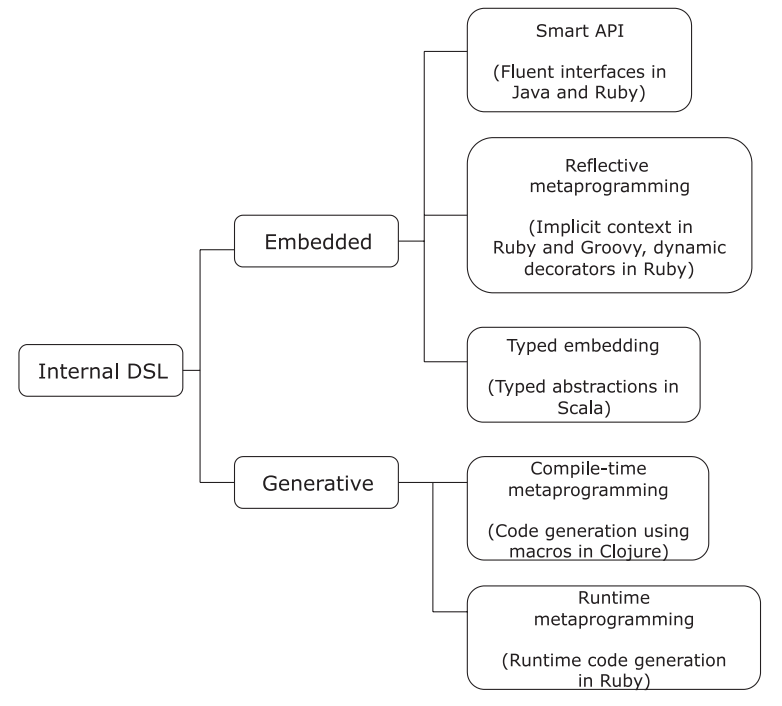
\includegraphics[width=0.8\textwidth]{images/DSLTechniques} 
      \caption{Internal DSL implementation techniques}
    \label{fig:DSLTechniques}
\end{figure}

Figure \ref{fig:DSLTechniques} shows the different kinds of implementation techniques for internal DSLs, as specified by \cite{Ghosh:2010}. Our DSL doesn't generate any code, so we won't discuss generative internal DSLs. for the JS-QL language, we use a \textit{smart API} approach, as it is ideal for our domain. By chaining methods in our DSL we can specify which states we want to encounter along the graph in a clearly specified order. We can define smart API as follows:

\begin{definition}
    \textit{a \textbf{smart API} is an API that is readable, easy to use and does not need boiler plate to work properly.}
\end{definition}

Readability is key for DSLs. Implementing a fluent interface is a way to improve readability and make a smart API. To this extend method chaining is a popular technique: It can be implemented by making the output of one method flow naturally as the input of another. Benefits are that a series of invocations in the DSL feel more natural and that it expresses the series of actions you want to perform or detect in the problem domain. 

\subsubsection*{Alternative approaches}

Alternative approaches for implementing embedded internal DSLs are reflective metaprogramming and type embedding.
We can already rule out type embedding, as this is only used for statically typed programming languages (JavaScript is dynamically typed). Reflective programming on the other hand would have been a good approach if we needed to add information to the states of the flow graph. However, JIPDA states are self-contained (they contain all necessary information) and they thus do not need additional individual functionality or information.

\subsection*{Used DSL design patterns}

Combining a smart API with several carefully chosen DSL design patterns\cite{DSLFowler} result in the concise and easily readable language that JS-QL is today. The remainder of this section elaborates on the chosen design patterns.

\subsubsection*{Method chaining}

Method chaining is a principle that allows methods to be specified one after another, and it is the bread and butter of our query language. This approach offers a fluent interface to the user with the aim to write readable queries and avoid coding mistakes. The ability to express a state one wishes to encounter as a chained method to states discovered earlier in the graph allows to build very readable queries.
\begin{exmp}
\label{ex:fluentInterface}
 Consider the query: \texttt{G.skipZeroOrMore().functionCall()}. It is obvious that this code is intuitive: \texttt{G} is the entry point of our language, which indicates the start of a query. We then search for a path in the graph that contains a function call somewhere down that path. This is expressed by \texttt{skip}ping zero or more states until a function call state is encountered.
\end{exmp}

\subsubsection*{Literal map}
%literal map
%-> Argument is a map similar to literal map
A literal map provides provides the functionality to let the user specify detailed key-value pairs.
Specifying that one wishes to find states is often too general. To this extent literal maps can be used to express which types of states we want to match and what information we want to capture in (meta)variables. 
\begin{exmp}
\label{ex:literalMap}
\texttt{functionCall(\{name: 'f', arguments: '?args'\})}. The literal map, enclosed in curly braces, indicates that only fuction calls with name \texttt{f} need to be matched and that the arguments of the matched state need to be captured in metavariable \texttt{?args}.
\end{exmp}

\subsubsection*{Object scoping}

Object scoping encapsulates the language in such a way that the effects of the language only reach within the scope of this object. The example for the method chaining design pattern is also applicable for the object scoping pattern. A single entry point \texttt{G} is created for queries, limiting the impact of the query that object. This pattern remedies two JavaScript flaws: Global namespace pollution and malicious code injection. Potentially malicious code will only harm the \texttt{G} object, which is contained in some sort of sandbox.

\subsubsection*{Deferred evaluation}
%deferred evaluation
%-> Used to specify extra properties (not available at compile-time) + filters on values that aren't available
Deferred evaluation postpones evaluation of certain expressions, such as function calls. Some queries in JS-QL contain definitions for extra properties and filters. The information for these filters and properties is often not available at compile-time of our language. Deferred evaluation is used as a technique to delay the evaluation of those filters and properties until the matching process in the backend has collected enough information. Our framework handles this by creating thunks for filters and properties and unwrapping these thunks when the matching engine needs to evaluate them. By the time the evaluation happens, all variables should be bound in these thunks in previous matching steps.
\begin{exmp}
Consider a metavariable \texttt{?val} which captures a value of an assignment. If we only want to match assignment states with a value greater than 2, we have to create a thunk for the filter function \texttt{>} with arguments \texttt{?val} and 2. We can not discard states with \texttt{?val} greater than 2 immediately, as we don't know which value will be bound to \texttt{?val} at compile time.
\end{exmp}

\subsubsection*{Delimiter directed translation}
The delimiter directed translation design pattern imposes that statements in the DSL are separated by a delimiter. These statements then are evaluated from left to right separately. As method chaining is used as a means to set up the JS-QL fluent interface, all methods are separated by a dot (the delimiter). Each method separated by this dot gets separately translated internally into a representation that is easier for our backend to process.

\subsubsection*{Newline separators}

Finally, the newline separators design pattern is incorporated in our DSL. This design pattern allows users to enter newlines between parts of their code. This greatly improves the readability and can split a program up in logical parts. Our DSL supports newlines in queries. This can be very useful to separate different states or sequences of states. Consider an example in which we only want to find assignments to variables \texttt{a} and \texttt{b}. Code can then be divided in two distinct parts, as in example \ref{ex:newlineSeparators}.

\begin{exmp}
\label{ex:newlineSeparators}
JS-QL code can be split up in logical parts thanks to its support for newline separators.
\begin{lstlisting}[label={lst:newlineSeparators},language=JavaScript,caption=Newline separators,mathescape=true]  % float=t?

.assign({leftName: 'a'}) //first logical part
.or()
.assign({leftName: 'b'}) //second logical part
\end{lstlisting}
\end{exmp}
%newline separators
%-> Language supports newlines between every state

%TODO conclusion?

\section{Existing DSL approaches for querying graphs}

In this section, we describe some existing approaches for querying graphs. We describe four external DSL approaches and three internal DSL approaches. The latter gave us inspiration to build our own JS-QL internal domain-specific query language.

\subsection{External DSLs}

Many DSLs come along with a compiler which translates DSL programs into applications. These kinds of DSLs are called \textit{external} DSLs. the compiler is also called an application generator\cite{Cleaveland:1988}, whereas the DSL is the application-specific language. The main advantage of external DSLs is that the implementation of the compiler can completely be tailored to the DSL. The DSL in turn is restricted in no way with regards to notation and primitives because its syntax is independent of any underlying host language. The remainder of this section discusses existing work about external DSLs used for graph traversal and graph querying.

\subsubsection*{StruQL}

StruQL is the query language behind the Strudel system\cite{Fernandez97aquery}. The language is built to support the retrieval and construction of data for web sites. This data is represented as \textit{data graphs} and originates from external sources, the integrated view and the web site itself. These data graphs depict web sites as graphs in which nodes represent web pages or atomic values and labelled edges which interconnecting nodes. These edges then represent the links or attribute values that connect two nodes. The language enables users to create and query data graphs, but the real power of StruQL lies in its ability to express regular path expressions. This allows for very flexible queries describing the paths about which information needs to be accessed in great detail.
It also allows to compute the transitive closure of an \textit{arbitrary 2n-ary} relation, meaning that it can compute all reachable nodes from a certain node for any input graph. 

\subsubsection*{GraphQL}
%http://sites.fas.harvard.edu/~cs265/papers/he-2008.pdf -> GraphQL

GraphQL\cite{He:2008} is a query language for querying graph databases. The language uses a graph pattern as a basic operational unit. These graph patterns consist of a graph structure and a predicate on attributes of the graph. GraphQL introduced the notion of formal languages for graphs. This is useful for composing and manipulating graph structures and is used as a basis of the graph query language.
The core of the language is a graph algebra in which the selection operator is generalized to graph pattern matching and a composition operator is introduced for rewriting matched graphs. In terms of expressive power, the language is contained in Datalog. This means that every query in GraphQL can be converted to a Datalog query. The language allows users to express concatenation, disjunction and recursion, allowing users to write dynamic queries. They address the NP-completeness of subgraph isomorphism by using neighborhood subgraphs and profiles, joint reduction of the search space, and optimization of the search order.

\subsubsection*{ASTLOG}
%http://www.cs.nyu.edu/~lharris/papers/crew.pdf
ASTLOG\cite{Crew:1997} is a query language for syntax-level C/C++ program analysis and is well suited to construct anchored patterns to match tree-like structures. Syntax-wise, the language is built as a Prolog variant, but instead of transforming an entire program into a database of Prolog rules, it is able to match \textit{objects} to queries directly. These objects are being made available through a C/C++ compiler frontend which provides an interface to the syntactic/semantic data structures built during the parse of a program. Among the available objects are the AST nodes of a program. These nodes can then be examined and queried by user-defined predicates in a similar fashion as one would do in Prolog. This allows for application-specific composable predicates. 

\subsubsection*{Lorel}
The Lorel language\cite{abiteboul1997lorel} was designed to query semistructured data. This kind of data can be seen as a graph with complex values at internal nodes, labeled edges and atomic leaves. The language's syntax resembles that of OQL (\textit{Object Query Language}), but has two two additional features: (i) A coercion mechanism for value/object comparisons and (ii) powerful path expressions. Coercion is needed for semistructured data, as two objects may represent the same data in different ways. Lorel introduces \textit{general path expressions}, a way to define label completion and regular expressions in paths. Regular expressions are supported through \texttt{.},\texttt{+},\texttt{?},\texttt{*},\texttt{()} and \texttt{|}, label completion is done as in SQL, namely with the \texttt{\%} symbol.
%http://infolab.stanford.edu/lore/pubs/lorel96.pdf -> Semistructured data

%-----------------------------
%RW over EDSL los van graphs:
%http://graphics.stanford.edu/hackliszt/liszt_sc2011.pdf
%http://homepages.cwi.nl/~jurgenv/papers/SCAM-2009.pdf
%https://www.researchgate.net/publication/220071161_BDL_A_Specialized_Language_for_Per-Object_Reactive_Control
%Chandra1999
%-----------------------------


\subsection{Internal DSLs}
 This section describes three internal DSLs, two for graph traversal and one that illustrates the flexibility and expressiveness of embedded DSLs. The terms internal DSL and embedded DSL both have the same meaning in the rest of this dissertation and both refer to the type of DSL that is embedded in a host language.

%Waarom internal
%----------------
%RW over DSEL graph traversal:
\subsubsection*{Gremlin}
%http://arxiv.org/pdf/1508.03843.pdf -> Graph traversal
the Gremlin~\cite{Gremlin} language is a graph traversal machine. The machine traverses graphs according to a user-specified traversal, making use of so-called traversers. These traversers can be seen as 'workers' who walk through the graph, maintining information about the path they have already taken and the current graph node they are in. The language is meant to be implemented as an internal DSL in a host language that supports \textit{function composition} and \textit{functions functions as first-class entities}. The Gremlin language has an \textit{instruction set} of about 30 steps and each query is a sequence of these steps (i.e. a path). Querying graphs through paths is a well-known approach, but the Gremlin machine also supports nested paths in which each nested path is a graph traversal on its own. Queries are transformed into traversals, so each traversal can be made application-specific. Gremlin present 9 different traversals, including a recursive and a domain-specific one. 

\subsubsection*{Dagoba}

Dagoba\footnote{http://aosabook.org/en/500L/dagoba-an-in-memory-graph-database.html} is an in-memory graph database system written in JavaScript. The chapter about Dagoba in the \textit{500 Lines or Less}\footnote{http://aosabook.org/en/500L} book provides an elaborate explanation on how to create a flexible, easily extensible internal DSL. The language is built as a fluent API, and explains which mechanics (such as lazy evaluation) go hand in hand with this kind of language representation. The developers of Dagoba also describe how they interpret the language and define some optimizations of the system, mainly through query transformators.

\subsubsection*{A little language for surveys}

A Little Language for Surveys \cite{RubyDSL} explores the use of the Ruby programming language to implement an internal domain-specific language. It checks how well the flexible and dynamic nature of the language accomodates for the implementation of a DSL for specifying and executing surveys. Two key features of the Ruby programming language are exploited because these features especially support defining internal DSLs: the flexibility of the syntax and the support for blocks. Function calls for example are easily readable, since the braces surrounding the arguments can be omitted and the argument list can consist of a variable number of arguments . They make extensive use of the fact that entire blocks can be attached to method calls. These blocks are passed unevaluated to the called method, enabling \textit{deferred evaluation}. In addition to these features, the meta-programming facilities of Ruby make it possible to read a DSL program and execute it in the contexts specified by that program. A two-pass architecture is used, splitting up the parsing and interpretation of the program. This is common practice for internal DSLs.


\section{Conclusion}
In this chapter we discuss our approach for building the JS-QL framework. We described the architecture of the framework and discussed each component. As our approach uses the JIPDA abstract state graph as a program presentation, we described the information that can be found in this graph. JS-QL is an embedded domain-specific language. In this chapter we motivated the use of an embedded DSL, and we describe the design constraints and design patterns that influenced the language. Finally, we provided an overview of existing DSL approaches for querying graphs.

